%\subsubsection{Sóng điện từ}
\subsubsection{Khái niệm}
\newghichu{Sóng điện từ là điện từ trường lan truyền trong không gian}
\begin{center}
\begin{tikzpicture}[scale=0.9,transform shape,x=(0:1.2), y=(90:1.0), z=(-150:1.0),
line cap=round, line join=round,
axis/.style={black, thick,->},
vector/.style={>=stealth,->},scale=1,thick,>=stealth']
\colorlet{myblue}{black!40!blue}
\colorlet{myred}{black!40!red}
\draw[dashed](-0.5,1.5)--(7.86,1.5)--(7.85,-1.5)--(-0.5,-1.5);
\draw[left color=gray,right color=gray,middle color=white](-0.25,1.5)--++(-90:3)arc(0:-180:0.4cm and 0.1cm)--++(90:3)--cycle;
\draw[left color=gray,right color=gray,middle color=white](-0.25,1.5)arc(0:360:0.4cm and 0.1cm);
\draw[->](-0.5,0.25)--++(90:0.75);
\draw[->](-0.7,1)--++(-90:0.75);
\node[rotate=90] at (-1.2,0.5){Chấn tử};

\large
\def\A{1.5}
\def\nNodes{5} % use even number
\def\nVectorsPerNode{8}
\def\N{\nNodes*40}
\def\xmax{\nNodes*pi/2*1.01}
\pgfmathsetmacro\nVectors{(\nVectorsPerNode+1)*\nNodes}
\def\vE{{\color{myblue}\mathbf{E}}}
\def\vB{{\color{myred}\mathbf{B}}}
\def\vk{\mathbf{\hat{k}}}
\def\drawENode{ % draw E node and vectors with some offset
\draw[myblue,very thick,variable=\t,domain=\iOffset*pi/2:(\iOffset+1)*pi/2*1.01,samples=40]
plot (\t,{\A*sin(\t*360/pi)},0);
\foreach \k [evaluate={\t=\k*pi/2/(\nVectorsPerNode+1);
\angle=\k*90/(\nVectorsPerNode+1);}]
in {1,...,\nVectorsPerNode}{
\draw[vector,myblue!50] (\iOffset*pi/2+\t,0,0) -- ++(0,{\A*sin(2*\angle+\iOffset*180)},0);
}
}
\def\drawBNode{ % draw B node and vectors with some offset
\draw[myred,very thick,variable=\t,domain=\iOffset*pi/2:(\iOffset+1)*pi/2*1.01,samples=40]
plot (\t,0,{\A*sin(\t*360/pi)});
\foreach \k [evaluate={\t=\k*pi/2/(\nVectorsPerNode+1);
\angle=\k*90/(\nVectorsPerNode+1);}]
in {1,...,\nVectorsPerNode}{
\draw[vector,myred!50] (\iOffset*pi/2+\t,0,0) -- ++(0,0,{\A*sin(2*\angle+\iOffset*180)});
}
}
% main axes
\draw[axis] (0,0,0) -- ++(\xmax*1.1,0,0) node[right] {$\vec{v}$};
\draw[axis] (0,-\A*1.4,0) -- (0,\A*1.4,0) node[right] {$\vec{E}$};
\draw[axis] (0,0,-\A*1.4) -- (0,0,\A*1.4) node[above left] {$\vec{B}$};
% draw (anti-)nodes
\foreach \iNode [evaluate={\iOffset=\iNode-1;}] in {1,...,\nNodes}{
\ifodd\iNode \drawBNode \drawENode % E overlaps B
\else \drawENode \drawBNode % B overlaps E
\fi
}
\draw(4.7,0)--(4.7,-2)(7.85,0)--(7.85,-2);
\draw[<->](4.7,-1.8)--node[midway,below]{Bước sóng}(7.85,-1.8);
%Vẽ đinh ốc
\begin{scope}[shift={(0,-1.1)}]
\draw[fill=white,rounded corners=0.6](0,-1.5)coordinate(a)--++(-45:0.5)coordinate(b)--++(0:1.2)--++(-45:0.1)coordinate(c)--++(0:2)--++(-20:0.5)--++(-160:0.5)--++(180:2)coordinate(d)--++(-135:0.1)--++(180:1.2)coordinate(f)--++(-135:0.5)--++(90:0.5)--++(0:0.15)--++(90:0.1)--++(180:0.15)--cycle;
\draw[fill=Mapcolor](a)++(-90:0.15)--++(-38:0.43)--++(0:1.2)--++(-45:0.1)--++(-90:0.05)--++(150:0.08)--++(180:1.2)--++(150:0.38)--cycle;
\draw[fill=Mapcolor](a)++(-90:1)--++(35:0.42)--++(90:0.05)--++(-155:0.37);
\draw(b)--(f)(c)--(d);
\foreach \x in {1.63,1.93,...,3.7}
\foreach \y in {-1.925}
{\draw[fill=Mapcolor,very thin](\x,\y)--++(60:0.1)--++(-60:0.1)--++(-75:0.35)--++(-120:0.1)--++(120:0.1)--cycle;
\draw[fill=white,very thin](\x,\y)--++(60:0.1)--++(-80:0.5)--cycle;
}
\draw[fill=Mapcolor,very thin](3.68,-1.96)--++(60:0.05)--++(-60:0.06)--++(-75:0.25)--++(-120:0.05)--++(120:0.05)--cycle;
\draw[fill=white,very thin](3.68,-1.96)--++(60:0.05)--++(-78:0.34)--cycle;
\draw[fill=Mapcolor,very thin](3.85,-2.01)--++(60:0.05)--++(-60:0.06)--++(-75:0.15)--++(-120:0.05)--++(120:0.05)--cycle;
\draw[fill=white,very thin](3.85,-2.01)--++(60:0.05)--++(-78:0.24)--cycle;
\end{scope}
\draw[->](4.5,-3.2)--++(0:1);
\draw[->](3.6,-2.7)arc(60:320:0.2cm and 0.6cm);
\end{tikzpicture}
\end{center}
\subsubsection{Tính chất của sóng điện từ}
\begin{itemize}
\item Sự lan truyền sóng điện từ:
\begin{itemize}
\item Sóng điện từ lan truyền được trong chân không với tốc độ bằng tốc độ ánh sáng $(c\approx3.10^{8}\ m/s)$. 
\item Sóng điện từ lan truyền được trong các môi trường khác với tốc độ $v=\dfrac{c}{n}$ với n là chiết suất môi trường. 
\end{itemize}
\item Sóng điện từ là sóng ngang. Trong quá trình lan truyền, vectơ cường độ điện trường \bth{\vec{E}} và vectơ cảm ứng từ $\vec{B}$ luôn luôn vuông góc với nhau và vuông góc với phương truyền sóng. 
\item Điện trường và từ trường trong sóng điện từ luôn cùng pha với nhau.
\item Sóng điện từ tuân theo quy luật truyền thẳng, phản xạ, khúc xạ, nhiễu xạ và giao thoa như ánh sáng.
\item Sóng điện từ mang năng lượng.
\end{itemize}
\immini{
%\subsubsection{Bước sóng. Các loại sóng vô tuyến}
\subsubsection{Bước sóng của sóng điện từ}
Bước sóng điện từ trong chân không: 
\begin{center}
$\boder{\lambda=\dfrac{c}{f}}$ 
\end{center}
\subsubsection{Tầng điện li}
\newghichu{
\textbf{Tầng điện li} là một lớp khí quyển, trong đó các phân tử khí đã bị ion hoá rất mạnh dưới tác dụng của các tia tử ngoại trong ánh sáng mặt trời.
}
}
{
\begin{tikzpicture}[scale=0.8,transform shape,thick,>=stealth']
\clip (-5,2) -- (-5,10) -- (5,10) -- (5,2)--cycle;
\tkzDefPoints{0/0/o}
\tkzDefShiftPoint[o](90:9){a}
\tkzDefShiftPoint[o](120:5.03){b}
\tkzDefShiftPoint[o](60:5.03){c}
\tkzDefShiftPoint[o](130:5.1){d}
\tkzDefShiftPoint[o](50:5.1){e}
\shade [inner color=blue, outer color=white, even odd rule] circle (6) circle (4.6);
\shade [inner color=white, outer color=blue!60, even odd rule] circle (6.1) circle (6);
\node[inner sep=0pt] (russell) at (o){
\includegraphics[width=10cm]{Hinh/Earth1}};
\node[inner sep=0pt] (russell) at (a){\includegraphics[width=1.5cm]{Hinh/satellite.pdf}};
\node[inner sep=0pt,rotate=30] (russell) at (b){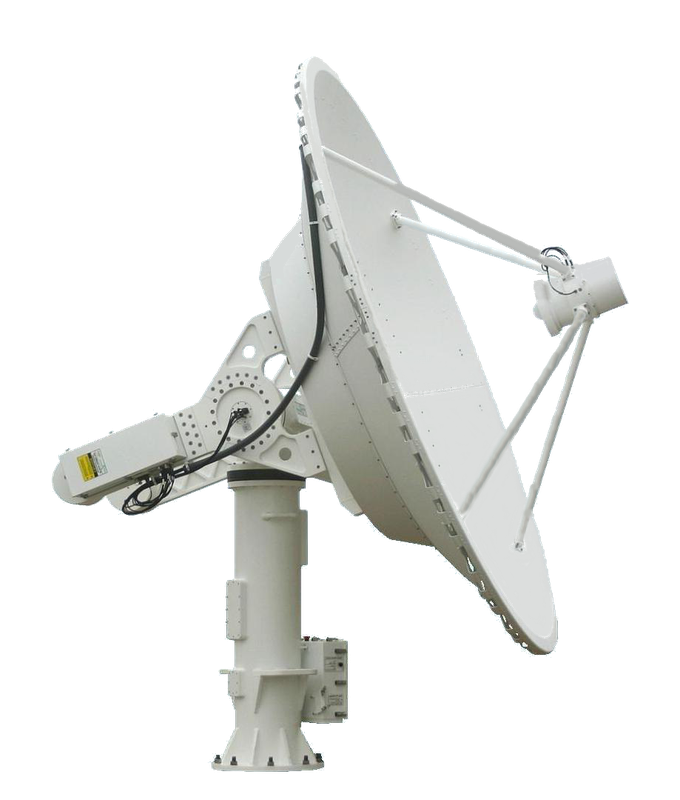
\includegraphics[width=0.8cm]{Hinh/Rada2}};
\node[inner sep=0pt,rotate=-30] (russell) at (c){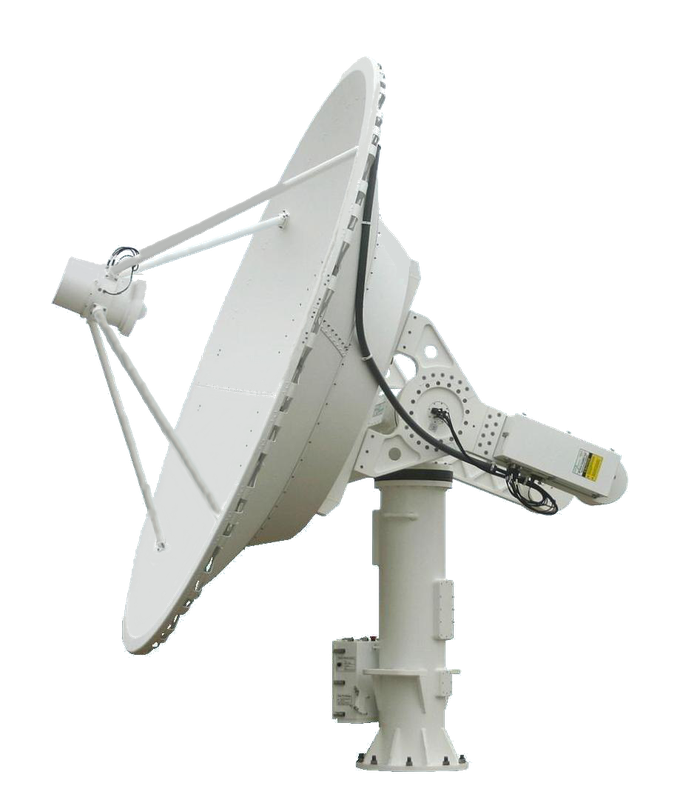
\includegraphics[width=0.8cm]{Hinh/Rada1}};
\node[inner sep=0pt,rotate=40] (russell) at (d){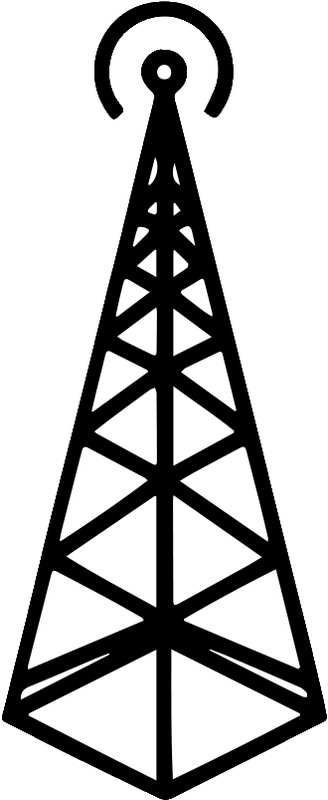
\includegraphics[width=0.5cm]{Hinh/CotPhatSong}};
\node[inner sep=0pt,rotate=-40] (russell) at (e){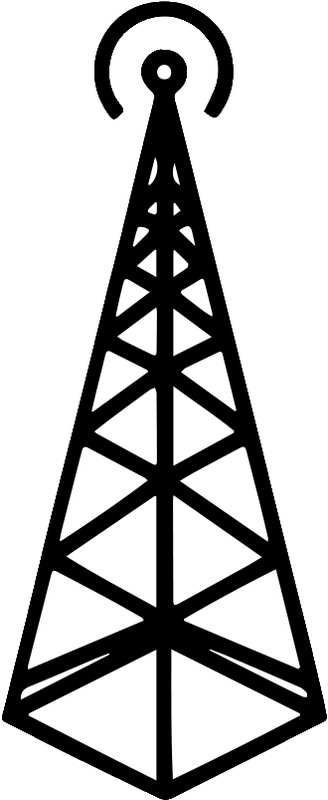
\includegraphics[width=0.5cm]{Hinh/CotPhatSong}};
\draw[dotted,line width=2pt,blue](b)--node[midway,above,sloped,black]{Sóng cực ngắn}(a)--node[midway,above,sloped,black]{Sóng cực ngắn}(c);
\begin{scope}
\tkzDefShiftPoint[o](130:5.6){f}
\tkzDefShiftPoint[f](22:4.5){f1}
\tkzDefShiftPoint[f](29:3.5){f2}
\clip (f) -- (f1) -- (f2) -- (f);
\foreach \x in {0.2,0.4,...,5}
{\draw[red,very thick] (f) circle (\x);}
\end{scope}
\begin{scope}
\tkzDefShiftPoint[o](50:5.6){f'}
\tkzDefShiftPoint[f](22:4.5){f1}
\tkzDefShiftPoint[f](29:3.5){f2}
\clip (f') -- (f2) -- (f1) -- (f');
\foreach \x in {0.2,0.4,...,5}
{\draw[red,very thick] (f') circle (\x);}
\end{scope}
\draw(-1,5.3)--++(-70:2)node[fill=white]{Sóng ngắn, trung, dài};
\node[]at (-3.8,3.6){Phát};
\node[]at (3.8,3.6){Thu};
\draw(a)++(0:0.7)node[right]{Vệ tinh};
\path[postaction={decoration={
text along path,text align=fit to path,
text format delimiters={|}{|},
text={|\fontsize{8}{8}\selectfont\bfseries| T{ầ}ng {đ}{i}{ệ}n l{i}},
text align=center,
reverse path
},
decorate}] (40:6.3cm) arc (40:70:6.3cm);
\end{tikzpicture}
}
\subsubsection{Sóng vô tuyến}
%\begin{longtable}{|p{0.15\textwidth}|p{0.25\textwidth}|p{0.25\textwidth}|p{0.25\textwidth}|}%[tabularx={X|X|X|X}]{Các loại sóng vô tuyến}
\begin{bang}[tabularx={l|X|X|X}]{Các loại sóng vô tuyến}
\hline
\textbf{Loại sóng}&\textbf{Bước sóng}&\textbf{Đặc điểm}&\textbf{Ứng dụng}\\\hline
\textbf{\textit{Sóng dài}}&$\geq 1000\ m$&Bị các vật trên mặt đất hấp thụ mạnh nhưng nước lại hấp thụ ít.&Dùng trong thông tin liên lạc dưới nước.\\\hline
\textbf{\textit{Sóng trung}}&$100\ m\to 1000\ m$&$\bullet$ Ban ngày bị tầng điện li hấp thụ mạnh.\newline
$\bullet$ Ban đêm bị tầng điện li phản xạ.&Dùng trong thông tin liên lạc vào ban đêm.\newline
\textit{Ban đêm nghe đài sóng trung rõ hơn ban ngày}\\\hline
\textbf{\textit{Sóng ngắn}}&$10\ m \to 100\ m$&$\bullet$ Có năng lượng lớn.\newline $\bullet$ Bị phản xạ nhiều lần giữa tầng điện li và mặt đất.& Dùng trong thông tin liên lạc trên mặt đất.
\\\hline
\textbf{\textit{Sóng cực ngắn}}&$0,01\ m\to 10\ m$&$\bullet$ Có năng lượng rất lớn. \newline $\bullet$ Xuyên qua tầng điện li vào vũ trụ.&Dùng trong thông tin vũ trụ và truyền hình vệ tinh.\\ \hline
%\end{longtable}
\end{bang}
\subsubsection{Các loại bức xạ}
\begin{bang}[tabularx={l|X|X|X}]{CÁC LOẠI TIA}
&\textbf{Tia hồng ngoại}
&\textbf{Tia tử ngoại}
&\textbf{Tia X (Rơn-ghen)}
\\\hline
\textbf{Định nghĩa}
&Tia hồng ngoại là các bức xạ không nhìn thấy có bước sóng \textbf{dài hơn} \bth{0,76\microm} đến vài khoảng milimet .
&Tia tử ngoại là các bức xạ không nhìn thấy có bước sóng \textbf{ngắn hơn} \bth{0,38\microm} đến cỡ $10^{-8}\ m$ .
&Bức xạ có bước sóng từ $10^{-11}\ m$ đến $10^{-8}\ m$.
\\\hline
\textbf{Nguồn phát}
&Mọi vật có nhiệt độ cao hơn 0 K đều phát ra tia hồng ngoại.
&
Các vật có nhiệt độ trên 2000\degree C: đèn hơi thủy ngân, hồ quang điện, mặt trời,\ldots\newline
%$\bullet$ Trong chùm ánh sáng Mặt Trời có 9\% năng lượng thuộc về tia tử ngoại.
&Dùng ống Cu-lit-giơ.
\\\hline
\textbf{Đặc điểm}
&
$\bullet$ Có tác dụng nhiệt mạnh.\newline
$\bullet$ Gây ra một số phản ứng hóa học, tác dụng lên một số loại phim ảnh.\newline
$\bullet$ Có thể biến điệu được như sóng điện từ cao tần.\newline
&
$\bullet$ Tác dụng mạnh lên phim ảnh, làm ion hóa không khí và nhiều chất khí khác.\newline
$\bullet$ Kích thích sự phát quang, gây ra một số phản ứng hóa học.\newline
$\bullet$ Bị thủy tinh, nước hấp thụ rất mạnh.\newline
$\bullet$ Hủy diệt tế bào da, làm hại mắt, diệt khuẩn, diệt nấm mốc,\ldots\newline
&
$\bullet$ Có khả năng đâm xuyên mạnh.\newline
$\bullet$ Có tác dụng mạnh lên phim ảnh, làm ion hóa không khí.\newline
$\bullet$ Có tác dụng làm phát quang một số chất.\newline
$\bullet$ Tia X có tác dụng sinh lí mạnh, hủy diệt tế bào, diệt vi khuẩn,\ldots
\\\hline

\textbf{Ứng dụng}
&
$\bullet$ Sưởi ấm, sấy khô quần áo,\ldots \newline
$\bullet$ Điều khiển từ xa.\newline
$\bullet$ Chụp ảnh bề mặt của Trái đất qua vệ tinh.\newline
$\bullet$ Ứng dụng đa dạng trong lĩnh vực quân sự.
&Khử trùng nước, thực phẩm và dụng cụ y tế, chữa bệnh (bệnh còi xương), tìm vết nứt trên bề mặt kim loại,\ldots
&
$\bullet$ Chiếu điện, chụp điện.\newline
$\bullet$ Kiểm tra chất lượng các vật đúc, tìm các vết nứt, các bọt khí bên trong các vật bằng kim loại.
\end{bang}
\subsubsection{Ánh sáng nhìn thấy}
\begin{itemize}
\item Dải bước sóng của ánh sáng nhìn thấy là một phần của thang sóng điện từ.
\item Quang phổ của ánh sáng nhìn thấy là một dải màu biến thiên liên tục từ tím $(\lambda_t=0,38\ \mu m)$ đến đỏ $(\lambda_{\text{đ}}=0,76\ \mu m)$.
\end{itemize}
\subsubsection{Thang sóng điện từ}
\begin{center}
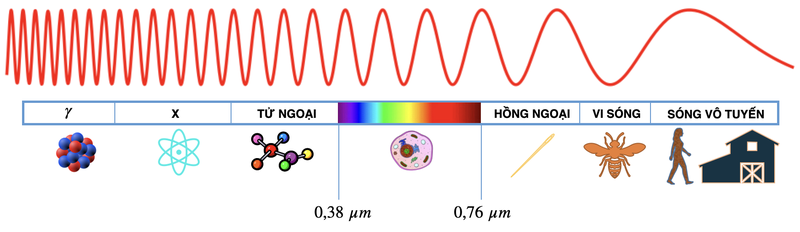
\includegraphics[width=12cm]{Hinh/songdientu}
\end{center}
\Binhluan{
Sóng vô tuyến, tia hồng ngoại, ánh sáng nhìn thấy, tia tử ngoại, tia Rơn-ghen, tia gam-ma có cùng bản chất là sóng điện từ. Chúng tạo thành dải bước sóng giảm dần (tần số tăng dần)}
{Các loại sóng điện từ \textit{không có một ranh giới nào rõ rệt.}}

